\documentclass[12pt,twocolumn]{article}
\usepackage[T1]{fontenc}
\usepackage{graphicx}
\usepackage{amsmath}
\usepackage[left=1cm,right=1cm,top=2cm,bottom=2cm]{geometry}
%\renewcommand*{\familydefault}{\sfdefault}
\title{\vspace{-2.5em}Investigation 2: 1D Diffusion}
\author{Christopher Pattison}
\date{}
\begin{document}
\maketitle
\section*{Derivation}
The Heat equation is discretized into a system of linear equations in the form $[A]\{x\}=\{b\}$
\[\nabla\cdot k\nabla T = q\]
In the Finite Volume Method, the equation is integrated over a control volume with finite 
differences used to approximate derivatives. A simplifying assumption is made that $k$ 
is invariant through the domain
\[\int_Vk\frac{d^2T}{dx^2} + q = 0\]
\[k\left.\frac{dT}{dx}\right\rvert_{x_w}^{x_e} + q(x_e-x_w)\]
\[k\frac{T_P-T_W}{x_P-x_W}-\frac{T_E-T_P}{x_E-x_P} + q(x_e-x_w)\]
\[\Delta x_e=x_E-x_P;\hspace{1em} \Delta x_w=x_P-x_W\]
\[k\frac{T_E\Delta x_e+T_W\Delta x_w-T_P(\Delta x_e + \Delta x_w)}{\Delta x_w \Delta x_e} + q(x_e-x_w)\]
The equation can then be put into the form
\[a_ET_E+a_PT_P+a_ET_E = q_P\]
A sparse coefficient matrix can then be formed for the domain
\[
\begin{bmatrix}
a_{11}&a_{12}&0\\
a_{21}&a_{22}&a_{23}\\
0&a_{32}&a_{33}
\end{bmatrix}
\begin{Bmatrix}
T_1\\T_2\\T_3
\end{Bmatrix}
=
\begin{Bmatrix}
q_1\\q_2\\q_3
\end{Bmatrix}
\]
A system solver can then be applied.
\begin{figure}
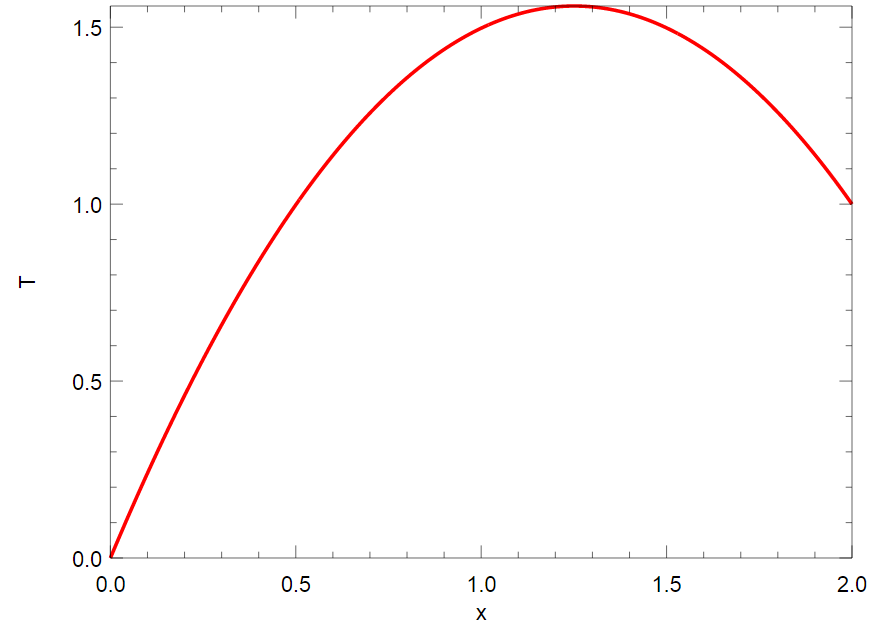
\includegraphics[width=\columnwidth]{result.png}
\footnotesize{\caption{Poisson's Equation in 1D}}
\end{figure}
\section*{Solvers}
Both Gauss-Jordan elimination and Gauss-Seidel methods were implemented on a dense matrix. The Gauss-Seidel 
implementation was over relaxed with a relaxation factor of 1.5 for comparison purposes. Notably, the direct solver was significantly faster than
over relaxed Gauss-Seidel for 1000 degrees of freedom. 
\section*{Convergence Improvement}
\subsection*{Over Relaxation}
Convergence of iterative solvers can be modified by multiplying the new solution vector by a relaxation factor $\omega \in (0,2)$.
Values less than 1 slow down convergence whereas values greater than 1 will increase convergence.
\[x^{k+1}=(1-\omega) x^k+ \omega D^{-1}(N x^k+ b)\]
Since the heat equation is unconditionally stable, a relaxation factor very close to 2 makes will improve convergence markedly. In testing, convergence speed was increased by over 10x.
\begin{figure}
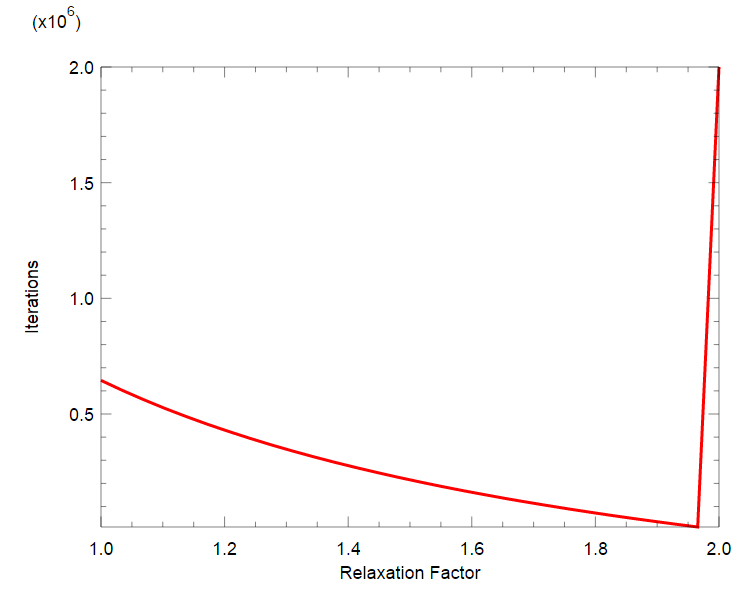
\includegraphics[width=\columnwidth]{sor.png}
\footnotesize{\caption{Relaxation Factor Iterations}}
\end{figure}
\subsection*{Multigrid}
Multigrid was implemented on top of the Gauss-Seidel solver
which reduced the number of iterations required drastically. Multigrid operates on the principle that information transfer through the domain
with most iterative methods is slow. To speed this up, the problem is solved on a coarse grid which is then mapped onto a successively finer grids,
increasing convergence speeds.
\paragraph{}The current Multigrid implementation uses a linear distribution of grid sizes from $\sqrt{\emph{DOF}}$ to DOF. 
After observing the convergence behavior, an improvement would be a power law distribution, refining the grid by perhaps 2x per evaluation until the full problem size is reached.
\section*{Possible Optimizations}
Significant optimizations were not made, however there is the potential for a few optimizations when the structure of the matrix is considered.
\subsection*{Gauss-Seidel}
An improvement to memory usage would be taking advantage of the tridiagonal structure of the coefficient matrix and
storing the non-zero terms only as in a sparse matrix storage scheme. Taking this a step further, since it is known that only the main
and adjacent diagonals will be non-zero, the matrix could be stored as a 3x\emph{N} array where \emph{N} is the number of 
degrees of freedom. The result is a reduction in memory usage to $O(N)$ as opposed to $O(N^2)$ for a naive storage scheme.
\begin{figure}
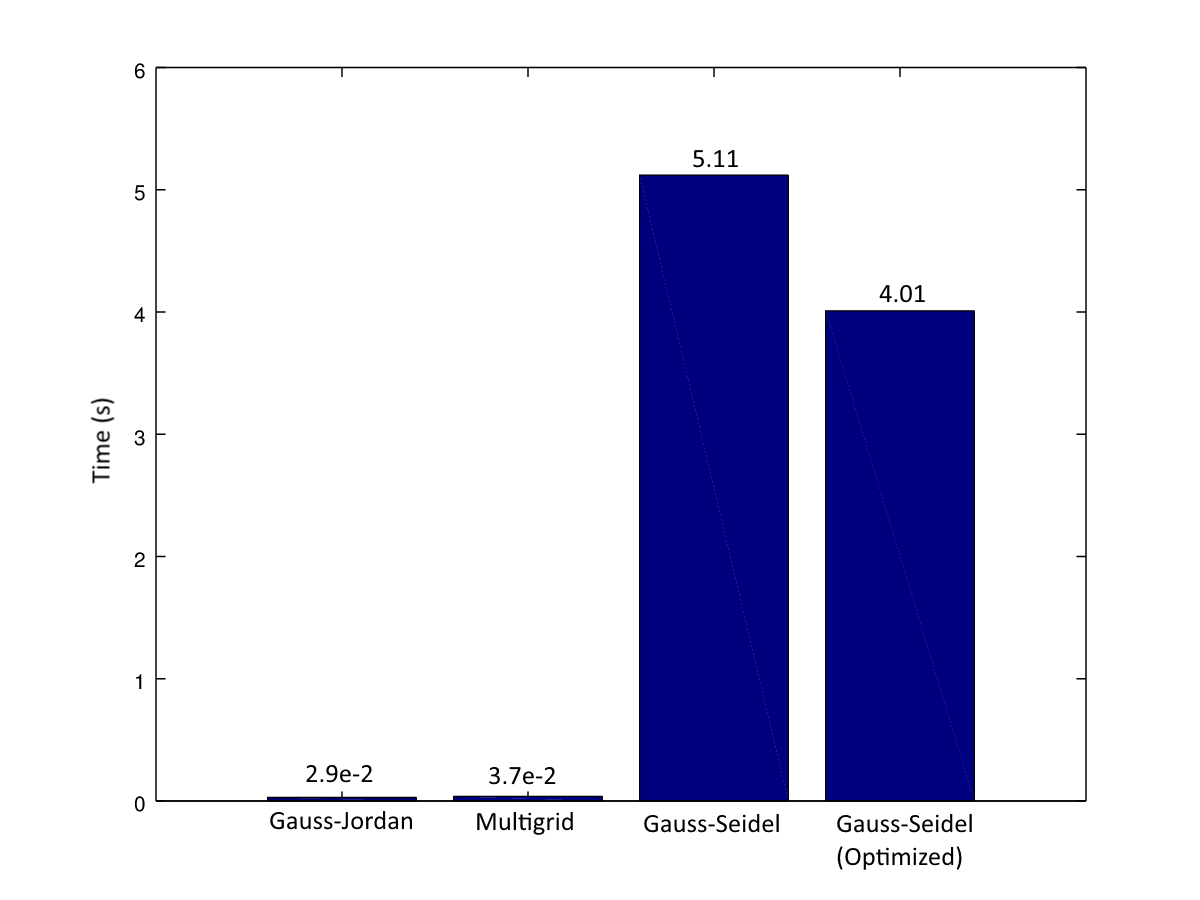
\includegraphics[width=\columnwidth]{bench.png}
\footnotesize{\caption{Solve Time}}
\end{figure}
\paragraph{}Another improvement to calculation speed would be to store the inverse of the diagonal coefficients. Computationally,
division is a very expensive operator taking nearly 20x the cycles as a multiply or add. A single unoptimized iteration 
of Gauss-Seidel for a tridiagonal matrix takes 28 cycles/DOF (8 add/multiply + 1 divide) for an in-order, non-vectorized processor.
By storing the inverse, the divide is changed to a multiply, reducing the cost of an iteration to 9 cycles/DOF (9 add/multiply), increasing theoretical throughput by over 3x. 
\paragraph{}Notably, the optimization resulted in only a 20\% speedup on a modern SandyBridge-E processor, suggesting that memory access is a large portion of the solve time once the problem is vectorized.
\subsection*{Gauss-Jordan}
The Gauss-Jordan solver does not take advantage of the sparsity of the matrix at all and assumes that the matrix is dense. This behavior 
could easily be improved by only carrying out necessary rows operations, changing the behavior from $O(N^2)$ to $O(N)$. An optimized version 
operating on a tridiagonal matrix would take 55 cycles/DOF (15 add/multiply + 2 divides) making it quicker than the iterative methods.
\end{document}
